\documentclass[a4paper,12pt]{report}
\addtolength{\oddsidemargin}{-1.cm}
\addtolength{\textwidth}{2cm}
\addtolength{\topmargin}{-2cm}
\addtolength{\textheight}{3.5cm}
\newcommand{\HRule}{\rule{\linewidth}{0.5mm}}
\makeindex

\usepackage{longtable}
\usepackage{graphicx}
\usepackage{makeidx}
\usepackage{hyperref}
\usepackage{verbatim}

\hypersetup{
    colorlinks=true,
    linkcolor=blue,
    filecolor=magenta,      
    urlcolor=cyan,
}


% define the title
\author{Team vbscript}
\title{ Assignment 2}
\begin{document}
\setlength{\parskip}{6pt}

% generates the title
\begin{titlepage}

\begin{center}
% Upper part of the page       
  
\textsc{\LARGE Department of Computer Science}\\[1.5cm]
\textsc{\Large COS 301 - Mini Project}\\[0.5cm]
% Title
\HRule \\[0.4cm]
{ \huge \bfseries Architectural Specification}\\[0.4cm]
\HRule \\[0.4cm]
% Author and supervisor
\begin{minipage}{0.4\textwidth}
\begin{flushleft} \large
\emph{Author:}\\
Tshepo {Malesela}\\
Mfana Masimula
Khodani Mufamadi
\end{flushleft}
\end{minipage}
\begin{minipage}{0.4\textwidth}
\begin{flushright} \large
\emph{Student number:} \\
u14211582\\
12077713\\
u14197520
\end{flushright}
\end{minipage}

\vfill

{\large \today}
\end{center}
\end{titlepage}
\footnotesize
\normalsize

\renewcommand{\thesection}{\arabic{section}}

\begin{center}
\tableofcontents
\footnotesize
\normalsize  
\end{center}

\renewcommand{\thesection}{\arabic{section}}
\newpage
\begin{center}
	\textsc{\LARGE Architectural Requirement Specification}\\[1.5cm]
	\textsc{\Large Team VbScript github repository link}\\[0.5cm]
	For further references see \href{https://github.com/mfanamasimula/VBScript}{gitHub}.
	\today
\end{center}
\newpage
\subsection{Architectural Scope}
\begin{itemize}
	\item The System should be accessable at anytime while the user is on campus.
	\item The server that host the system and the database is always on.
	\item The ability to navigate a given destination on campus
	\item The system must know your current location.
	\item The system must be able to to give ...
	\item The system need to be able to host all the users on campus.
	\item Administrative users have more access to the system have CRUD capabilties on events.
	\item Each event on the system must have a destination and multiple ways of reaching that destination through the navigation.
	\item The system must have the ability to notify users of current event.
	\item Users have the ability to set a route based on user constraints such as routes with less pedestrian trafic. 
\end{itemize}
\newpage
\subsection{External Interface Requirements}
	\subsubsection{User Interface}
		\begin{itemize}
			\item Standards for ...\\
			
			Fonts -  Verdana \\
			Images - square, ratio 1:1 \\
			Buttons labels - Button( HTML input element ) , LinkButton and ImageButton \\
			Color schemes - UP Colors , white , blue and red \\
			Field tabbing sequence - row by row \\
			
			\item Standard buttons, functions and navigation links that will
			appear on every screen. \\
			
				- Help button \\
				- Search button \\
				- Users: Login / Logout link \\
				- Navigation: always display users current location. \\
				- Events: button to navigate to current events on campus. \\\\
				
			\item Shortcut keys.\\
			
				Mobile Devices ( Android / iOS )  
				\begin{itemize}
					\item Volume UP = Open textbox to search New direction
					\item Volume DOWN = View events on campus 
				\end{itemize}
				    
				Desktop Computer
				\begin{itemize}
					\item Ctrl + F = Open textbox to search New direction
					\item Ctrl + E = View events on campus 
					\item Ctrl + Z = logout / logOff
					\item Ctrl + Alt + H = Help
	
				\end{itemize}
				
			\item Message dispaly conventions \\
				- Dialog box: Error message , usage/help message \\ 
				- Notification icon: 
				\begin{itemize}
				\item Display on login, if user have not subscribe to recieve  notifications either via SMS or email.
				\item Alert user if any new events have been added or is about to take place.
				\end{itemize}
			
				- Status bar: Dispaly users current location at all times. \\
			
			\item Accommodation for visually impaired users.\\
			
				1.) Allowances For Enlarged Text: Stylesheet with large font size whose layout does not break 
				when text-only zoom is enabled in browser. \\
				
				2.) Use Keyboard Shortcuts to Aid Navigation: Possibly being able to nevigate the whole application 
				with the use of only shortcut keys. \\
				
				3.) Contrast is Key: Bold text on low contrust items and user ability to highlight text with mouse 
				( quick trick to increase contrast and to aid visual focus ). \\
		
		\end{itemize}
	\subsubsection{Hardware Interface}
		\begin{itemize}
		\item Supported Device type \\
		- WiFi supported divice \\
		- Precise location (GPS and network-based) support \\
		\item Data and control interaction between the software and hardware \\ 
		
	
		\item Communication protocol \\
		- 
		- JSON (JavaScript Object Notation) \\
		- Ajax (Asynchronous JavaScript and XML) \\
		\end{itemize} 
	\subsubsection{Software Interface}
		\begin{itemize}
			\item Databases: \\
			- Databases: MongoDB \\
			- Operating Systems:  \\
			
			\item Operating Systems: \\
			Mobile devices: \\
			- Android 4.2 (Jelly Bean) or later \\
			- iOS 8 or later \\
			
			Desktop:\\
			- accessible through Web browsers ( Google chrome or Mozilla Firefox ) @www.nav.up.ac.za 
			
			
		\end{itemize}
		
		
		 
	\subsubsection{Communicatons Interface}
\newpage
\subsection{Performance Requirements}
	
		\subsubsection{Response Time}
		Support 90000 Guests, users and admin.\\
		Users consisting of students, lectures, and university employees.\\
		The system should be able to withhold the following performance requirement:\\
		- 95 percent of all the time (excluding Route Navigation response) the system should respond within 5 seconds.\\
		- Less than 10 seconds response time for normal expected route navigation during more than 60 percent of the 
		time as depicted by conditions on campus.\\
		- Atmost 20 seconds allocated for Route Navigation response time, at which Error messages for system failure are
		issured eg "Navigation taking longer then expected"
		
		\subsubsection{Workload}
		\begin{table}[h!]
			\centering
			\caption{User scenario statistics.}
			\label{tab:table1}
			\begin{tabular}{|c|c|c|c|}
				 \hline
				Scenario & Daily Total & Pages & Think Time \\
				\hline
				New user/Guest & 500 & Register, Login & 1 min \\
				\hline
				Looking for fun & 2500 & Events, Navigation & 25 seconds\\
				\hline
				Touring Campus & 150 & Points of interest, Navigation & 25 seconds \\
				\hline
				Lost on Campus & 4500 & Navigation & 15 seconds\\
				\hline
			\end{tabular}
			
			\bigskip
			Figure : User Traffic \\
			\begin{tabular}{l}
				
				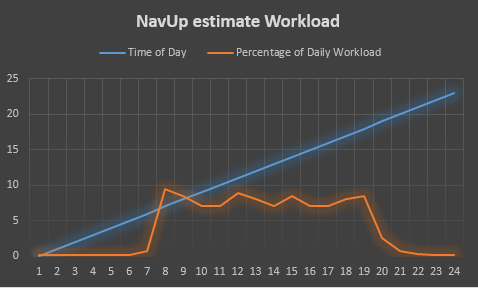
\includegraphics{workLoad.png}
				
			\end{tabular}
		
		\end{table}
	
		
		\subsubsection{Platform}
		 Not specific. Open to all systems that have WiFi support integration with functional requirement to enable 
		 GPS ( Global Positioning System ) operations. This include standard navigation features such as good graphics 
		 card for mapping directions in anyformat 2 or 3 dimensonal. 

\newpage
\subsection{Design Constraints}
\newpage
\subsection{Software System Attributes}
\newpage
\subsection{UML Design}
\subsubsection{Domain Model}
\subsubsection{Package Diagrams}
\textbf{Navigation Module} \\
\textbf{Events}\\
\textbf{Notification Module}\\
\textbf{GIS Module}
\subsubsection{Class diagrams}
\textbf{Navigation Module}\\
\textbf{Events}\\
\textbf{Notification Module}\\
\textbf{GIS Module}
\subsubsection{Package Diagrams}
\textbf{Navigation Module}\\
\textbf{Events}\\
\textbf{Notification Module}\\
\textbf{GIS Module}
\subsubsection{Activity Diagrams}
\textbf{Navigation Module}\\
\textbf{Events}\\
\textbf{Notification Module}\\
\textbf{GIS Module}\\

\newpage
\subsection{Design Patterns}
\newpage
\subsection{Technology}
Choosing the correct technologies is very important for this project because there may be  more than one way of performing a task but choosing the correct method can have other benefits such as better performance.
For this project the technologies have been devided into three categories, The Mobile technologies, The Server-Side Back End technologies, The Website Front-End technologies.
\subsubsection{Server-Side Back End Technologies}
\begin{itemize}
	\item CodeIgniter to provide a MVC framework to help with the development.
	\item MySQL which will be used to store the system data that will be queried later on.
	\item MongoDB for the system database and willbe used corrospondingly with the MYSQL
	\item PHP will be the server script language to be used in this project.
	\item Linux operating system on the server.
	\item Apache for the web server 
\end{itemize}
For this project requires reliability, security and performance and the solution of using LAMP (Linux, Apache, MySQL, PHP) which is a certified system with less weakness than more recent back end packages. LAMP  is also the ideal choice whhen you look at which languages the students a familiar with.
\subsubsection{Website Front-End Technologies}
\begin{itemize}
	\item HTML 5 to define the stucture and content of the website.
	\item CSS3 for the styling of the website and to provide animation where needed.
	\item Javascript to provide the website with functionality. The javascript will be used to process the return data from server.
	\item JQuery will be used with the javascript to provide functionality.
\end{itemize}

\subsubsection{Mobile Application Technologies}
\textbf{Android Application Technologies}
\begin{itemize}
	\item Android studio will be the platform for development.
	\item Java EE will be used as the programming language with the correct API's.
	\item RoboGuice to provide dependancy injection framework for android.
	\item GSON for converting Java objects to JSON representation and vice versa.
\end{itemize}
A native android application because native android applications provide some of the fastest performance and user interface. Building a native android application will help with how devices may display and content placement. If we are indeed building a native android application, Java will be the primary programming language.\\\\
\textbf{iOS Application Technologies}
\begin{itemize}
	\item Xcode 8/9 as the platform of development.
	\item Swift3 which is the programming language used to develop Apple applications.
	\item Objective C will be used inline with the Swift for developing apple applications.
	\item MapKit framework for providing a map we can change and all the map functionality.
	\item OpenGL ES GL Kit for the rendering of the systems interface, this will help with the graphics and look of the application.
\end{itemize}
These form the standard procedure for iOS application development.
\newpage
\subsection{Quality and Feasability Design}
\end{document}
